\documentclass[a4paper]{report}
\usepackage[margin=1in]{geometry}

\usepackage{graphicx}
\usepackage{hyperref}

\graphicspath{{./cn_images}}

\hypersetup{
    pdfborder = 0 0 0
}

\title{\textbf{\Huge Computer Networks Lab\\[10pt]
Network Simulator Project}}
\date{}



\begin{document}
    \maketitle
    % \oddsidemargin=0in

    \section*{\underline{Members}}
    \begin{tabbing}
        \hspace{1cm}\=Alwin C Sheejoy\quad\=-\quad\=7\kill
        \>  Adithyan M V        \>  -   \>  5   \\
        \>  Akshaylal S         \>  -   \>  6   \\
        \>  Alwin C Sheejoy     \>  -   \>  7   \\
        \>  Bharathan           \>  -   \>  21  \\
        \>  Jinso Raj           \>  -   \>  32  \\
        \>  Rohit               \>  -   \>  54  \\
    \end{tabbing}




    \section*{\underline{Problem Statement}}
    An organization is granted a network address 192.168.14.0. They need 14
    subnets. Design the subnet and implement dynamic routing between the
    fourth and seventh subnet using the network simulator NS3.\\




    \section*{\underline{Subnetting}}
    
    \begin{ttfamily}
        \begin{tabbing}
            subnet mask\quad\=:\quad\=255.255.255.240\kill
            ip address      \>  :   \>  192.168.14.0\\
            subnet mask     \>  :   \>  255.255.255.240\\[10pt]
            Subnet 4 \quad\= 192.168.14.48\quad\= - \quad\= 192.168.14.63\\
            Subnet 7 \> 192.168.14.96 \> - \> 192.168.14.111\\
            Router \> 192.168.14.240 \> - \> 192.168.14.255\\
        \end{tabbing}
    \end{ttfamily}



    \section*{\underline{Implementation Details}}
    \begin{ttfamily}
        \begin{tabbing}
            \underline{Router 1}\\[5pt]
            \hspace{1cm} \= fa0/0 \quad\= : \quad\= 192.168.14.49\\
            \> se0/0 \> : \> 192.168.14.241\\[5pt]
            \> R1\#config terminal\\
            \> R1(config)\#int fa0/0\\
            \> R1(config-if)\#ip address 192.168.14.49 255.255.255.240\\
            \> R1(config-if)\#exit\\
            \> R1(config-if)\#no shut\\
            \> R1(config)\#int se0/0\\
            \> R1(config-if)\#ip address 192.168.14.241 255.255.255.240\\
            \> R1(config-if)\#clock rate 64000\\
            \> R1(config-if)\#no shut\\
            \> R1(config-if)\#exit\\
            \> R1(config)\#router rip\\
            \> R1(config-router)\#network 192.168.14.48\\
            \> R1(config-router)\#network 192.168.14.240\\[25pt]

            \underline{Router 2}\\[5pt]
            \> fa0/0 \> : \> 192.168.14.97\\
            \> se0/0 \> : \> 192.168.14.242\\[5pt]
            \> R2\#config terminal\\
            \> R2(config)\#int fa0/0\\
            \> R2(config-if)\#ip address 192.168.14.97 255.255.255.240\\
            \> R2(config-if)\#no shut\\
            \> R2(config-if)\#exit\\
            \> R2(config)\#int se0/0\\
            \> R2(config-if)\#ip address 192.168.14.242 255.255.255.240\\
            \> R2(config-if)\#no shut\\
            \> R2(config-if)\#exit\\
            \> R2(config)\#router rip\\
            \> R2(config-router)\#network 192.168.14.96\\
            \> R2(config-router)\#network 192.168.14.240\\
        \end{tabbing}
    \end{ttfamily}


    \section*{\underline{Design Diagram}}
    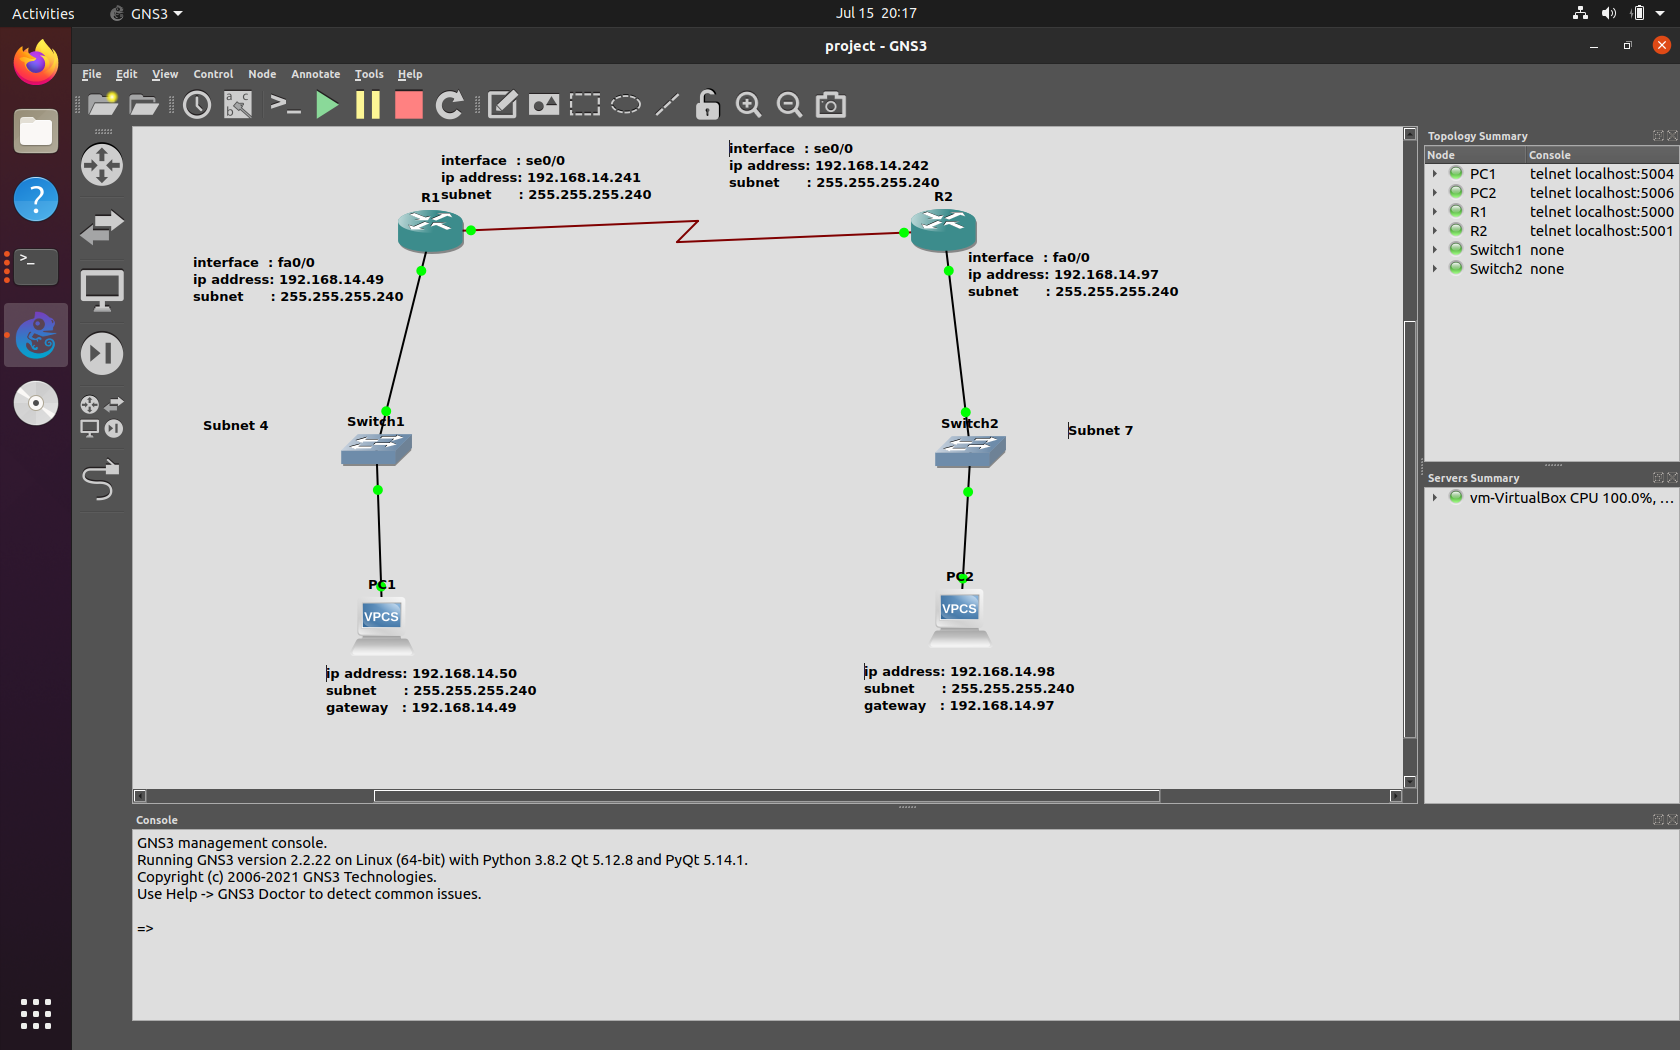
\includegraphics[width=16cm, height=10cm]{design.png}

    \section*{\underline{Output Screen}}
    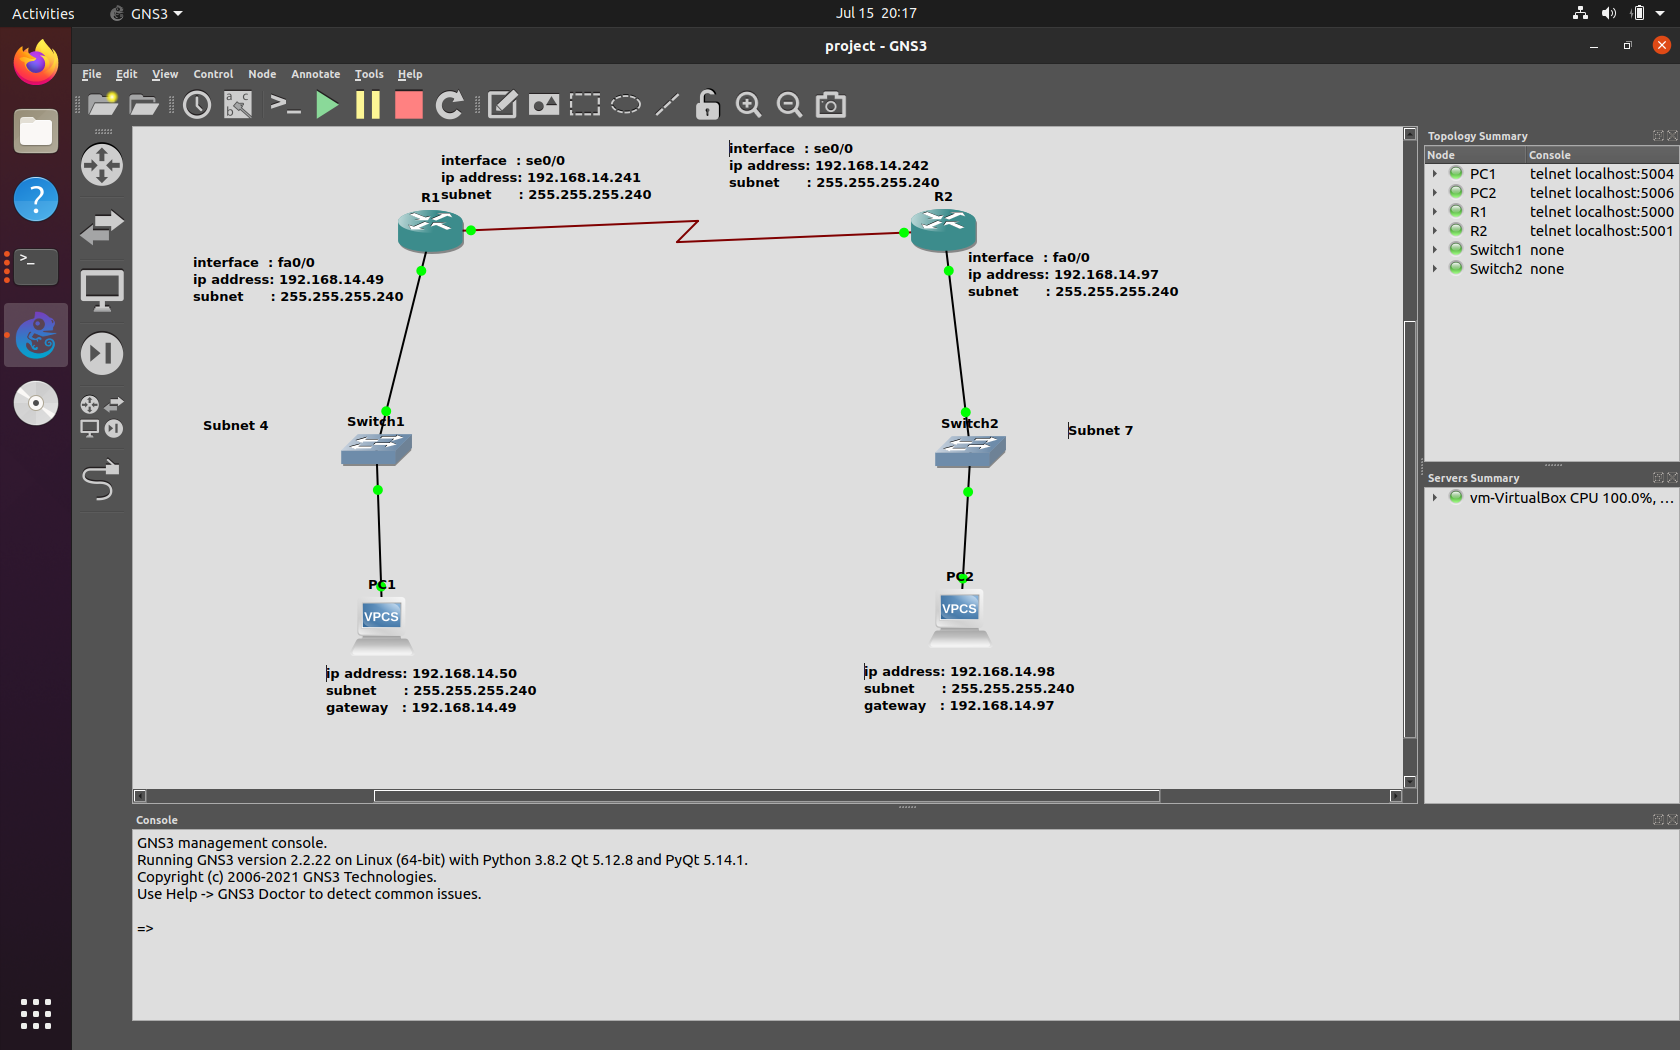
\includegraphics[width=16cm, height=10cm]{design.png}

    
\end{document}